\chapter{Background}
In this chapter, we will discuss the definitions
of the counting and point process. After that, we build up to the non-homogeneous Poisson process. However, we only present some definitions for the one-dimensional case are given, though many of these processes have a natural extension to higher dimensions.
\section{Counting and point processes}
Since Hawkes process is a special type of counting process, we will define what a counting process is. We will study the properties of counting process, which will lead into the definition of Hawkes process.

\begin{Definition}[{\cite[pp.3]{Hawkess}}(Counting process)]
	A counting process is a stochastic process $(N(t):t \geq 0)$ taking values in
	$N_{0}$ that satisfies $N_{0} = 0$, is finite, and is a right-continuous step function
	with jumps of size +1. Say that $(H(u) : u \geq 0)$ is the history of the arrivals
	up to time $u$.
\end{Definition}

A counting process can be viewed as a cumulative count of the number of ‘arrivals’ into a system up to the current time. Another way to characterise such a
process is to consider the sequence of random arrival times $T = \{T_{1}, T_{2}, . . .\}$ at which
the counting process $N(.)$ has jumped. The process defined as these arrival times is
called a point process, described in Definition \ref{Def Point process} (adapted from Carstensen 2010); see Fig. \ref{PointAndCountingProcess} for an example point process and its associated counting process.

  \begin{figure}[H]
  	\centering
  	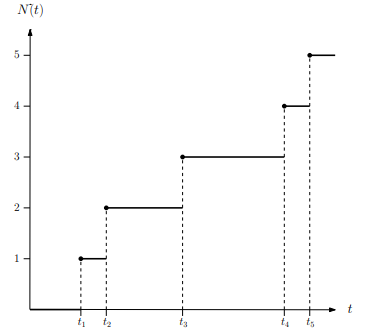
\includegraphics{PointProcessAndCountingProcess.PNG}
  	\caption{An example point process realisation $\{t_{1}, t_{2}, . . . \}$ and corresponding counting process $N(t)$.}
  	\label{PointAndCountingProcess}
  \end{figure}

To be able to fully understand what a counting process is, a point process must be defined. In this section, we introduce the fundamentals of point process. They are a foundation on which we build in later sections as the Hawkes process.

\begin{Definition}[{\cite[pp.3]{Hawkess}}(Point process)]{}	
If a sequence of random variables $T = {T_{1}, T_{2}, . . . }$, taking values in $R^{+} \cup {\infty}$, has: $P(0 < T_{0} \leq T_{1} \leq T_{2} \leq . . . ) = 1, P(T_{i} < T_{i+1}, T_{i} < \infty) = P(T_{i} < \infty) $ for $i \geq 1 $, and the number of points in a bounded region is finite almost surely (a.s.), then T is a (simple) point process.
\label{Def Point process}
\end{Definition}

The simplest point process is a Poisson process which some events arrive randomly with the constant intensity $\lambda$. This initial model describes sufficiently the simple process. For a example, the arrival of cars on a street over a short period of time. However, we need to vary the intensity event by the time $t$ to describe more complex processes such as simulating the arrivals of cars during rush hours and off-peak times. In a non-homogeneous Poisson process, the rate of event arrivals is a time function, i.e. $\lambda = \lambda(t)$.

\section{Non-homogeneous Poisson processes}
\begin{Definition}[{\cite[pp.5]{Hawkess}}(Non-homogeneous process)]{}	
Say a process $(N(t): t\geq 0)$ is a counting process and that it satisfies $ \forall s <t $ that $N(t)-N(s)$ is independent of $N(s)$ and that		
	\begin{align*}
	P(N(t + h) - N(t) = m \rvert N(t)) = 
	\begin{cases*}
	\lambda(t)h & $m = 1$ \\
	o(h) & $m > 1$  \\
	1-\lambda(t)h + o(h) & $ m = 0$  
	\end{cases*}  
	\end{align*}
then $N(t)$ is called a non-homogeneous Poisson process with $\lambda$ : $ R^{+} \rightarrow R^{+} $ called the intensity function; though if $\lambda(t) = \lambda $ for all $t \geq 0$, $N(t)$ is a homogeneous Poisson process.
\end{Definition}
However, a non-homogeneous Poisson process is only governed by an intensity function. One way to characterise a particular point process is to specify the distribution function of the next arrival time which bases on the past. The conditional intensity function is a convenient and intuitive way of specifying how the present depends on the past in an evolutionary point process.
\section{Conditional intensity functions}
\begin{Definition}[{\cite[pp.6]{Hawkess}}(Conditional intensity function)]{}	
Consider a counting process $N(.)$ with associated histories $H(.)$. If a function $\lambda^{*}(t)$ exists such that
 $$\lambda^{*}(t)= \lim_{h \to 0} \dfrac{E[N(t + h)-N(t) |H(t)]}{h}$$
that only relies on information of $N(.)$ in the past, then it is called the
conditional intensity function of $N(.)$.
\end{Definition}
